\subsection{The Millisecond Pulsar Gamma-Ray Luminosity Function}
\label{sec:glf}

For the gamma-ray luminosity function of MSPs, we adopt a log-normal parameterization:
%
\begin{align}
\frac{dP}{dL_{\gamma}}(L_{\gamma}) = \frac{1}{L_{\gamma} \sigma_L \sqrt{2\pi}} \exp\bigg(-\frac{(\ln L_{\gamma} - \ln L_0)^2}{2 \sigma_L^2}\bigg),
\label{eq:lumfunc}
\end{align}
%
where $L_0$ and $\sigma_L$ characterize the center and width of this distribution, respectively. We will often refer to this luminosity function in terms of the mean luminosity, which is given by $\langle L_{\gamma} \rangle = L_0 \, e^{\sigma_L^2/2}$.

The luminosity function of a globular cluster that contains a single MSP is simply equal to the expression given in Eq.~\ref{eq:lumfunc},
%
\begin{align}
\frac{dP}{dL_\textrm{tot}} (L_\textrm{tot}, N_\textrm{MSP}=1) = \frac{dP}{dL_{1}}(L_1=L_\textrm{tot}). 
\end{align}
%
For a cluster with two MSPs, $N_\textrm{MSP}=2$, it is instead given by
%
\begin{align}
\frac{dP}{dL_\textrm{tot}}(L_\textrm{tot}, N_\textrm{MSP}=2) =  \int_0^{L_\textrm{tot}} \frac{dP}{dL_1}(L_1) \, \frac{dP}{dL_2}(L_2=L_\textrm{tot}-L_1) \, dL_1,
\end{align}
%
and for $N_\textrm{MSP}=3$,
%
\begin{align}
\frac{dP}{dL_\textrm{tot}}(L_\textrm{tot}, N_\textrm{MSP}=3)  = \int_0^{L_\textrm{tot}-L_1} \int_0^{L_\textrm{tot}} \frac{dP}{dL_1}(L_1) \, \frac{dP}{dL_2}(L_2) \,\frac{dP}{dL_3}(L_3=L_\textrm{tot}-L_1-L_2) \, dL_1 \, dL_2,
\end{align}
%
and so on.

For a globular cluster containing a given mean number of expected MSPs, $\langle N_\textrm{MSP}\rangle$, its gamma-ray luminosity function will be given by
%
\begin{align}
\frac{dP}{dL_\textrm{GC}}(L_\textrm{GC},\langle N_\textrm{MSP}\rangle)  = \sum_{N_\textrm{MSP}=0}^\infty P(N_\textrm{MSP}) \, \frac{dP}{dL_\textrm{tot}}(L_\textrm{tot}, N_\textrm{MSP}),
\label{eq:glf}
\end{align}
%
where 
%
\begin{align}
P(N_\textrm{MSP},\langle N_\textrm{MSP}\rangle)= \frac{\langle N_\textrm{MSP}\rangle^{N_\textrm{MSP}} \, e^{-\langle N_\textrm{MSP}\rangle}}{N_\textrm{MSP}!}
\end{align}
%
is the Poisson probability that the globular cluster will contain $N_\textrm{MSP}$ pulsars.


In order to constrain the gamma-ray luminosity function of MSPs in globular clusters, we closely follow the analysis from Ref.~\cite{Hooper:2016rap}. 
We repeat these steps here for clarity:
\begin{enumerate}
    \item For a single globular cluster, $i$, we fit the energy spectrum to the Fermi-LAT data, as detailed in Section \ref{sec:fermi-data-analysis}. This gives us the observational likelihood profile for the flux, $\phi_i$, which we can write as $\mathcal{L}_{obs}(\phi_i)$. This function quantifies the measurement uncertainty of the flux.
    \item  We define the theoretical model for the gamma-ray luminosity function as in Eq.~\ref{eq:glf}. This is a probability density function  for the luminosity, $L_{\textrm{GC}, i}$, which depends on a set of model parameters which we call $\theta$.  We write this dependence explicitly as $p(L_{\textrm{GC}, i}|\theta)$.
    \item Given the relation between the flux and luminosity, $\phi_i = L_{\textrm{GC},i}/4\pi d_i^2$, where $d_i$ for each globular cluster is given in Table \ref{tab:tab7-9-hopper-linden}, it is possible to rewrite the luminosity function as function of the flux: $p_i(\phi_i|\theta)$. While the parameters $\theta$ would not depend on the specific globular cluster, the distance $d_i$ does. For this reason, given a gamma ray luminosity function, $p_i(\phi_i|\theta)$ will be different for each globular cluster.
    \item We combine the likelihood derived for a specific observation with the probability to observe a certain flux, and marginalize (integrate) over the flux in order to obtain the likelihood as a function of the parameter $\theta$: $\mathcal{L}_\textrm{obs}^i(\theta)=\int_0^\infty \mathcal{L}_\textrm{obs}(\phi_i)p_i(\phi_i|\theta)d\phi_i$
    \item We notice how each observation is independent from each other. For this reason, the joint likelihood on the entire set of globular clusters adopted in the analysis will be given by $\mathcal{L}_\textrm{obs}(\theta)=\prod_i \mathcal{L}_\textrm{obs}^i(\theta)$.
    \item Given the likelihood of the entire dataset $\mathcal{L}_\textrm{obs}(\theta)$, it is now possible to derive a maximum likelihood estimation of the parameters $\theta$.
\end{enumerate}
%%



\begin{figure}[t]
\centering
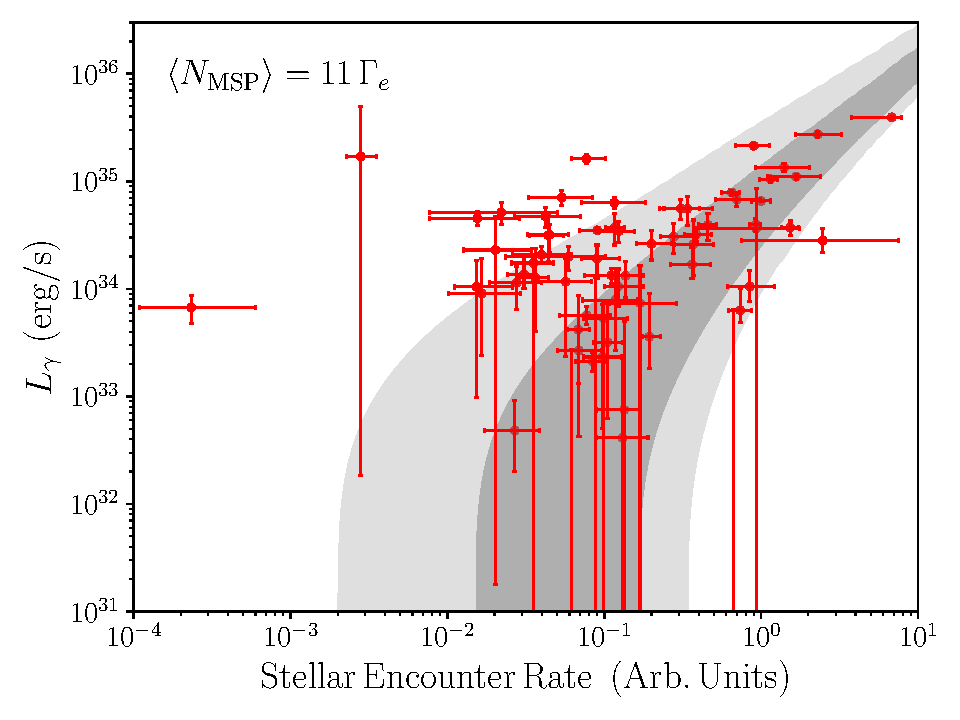
\includegraphics[width=0.49\textwidth]{sections/paper_msp/img/case1-dataplot.pdf}
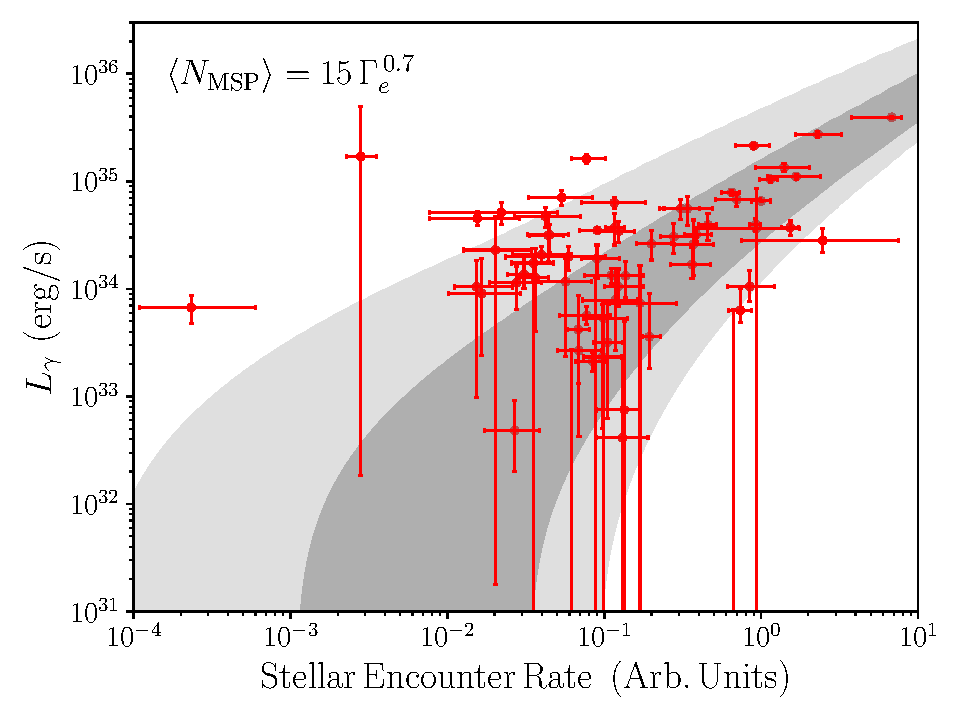
\includegraphics[width=0.49\textwidth]{sections/paper_msp/img/case2-dataplot.pdf}
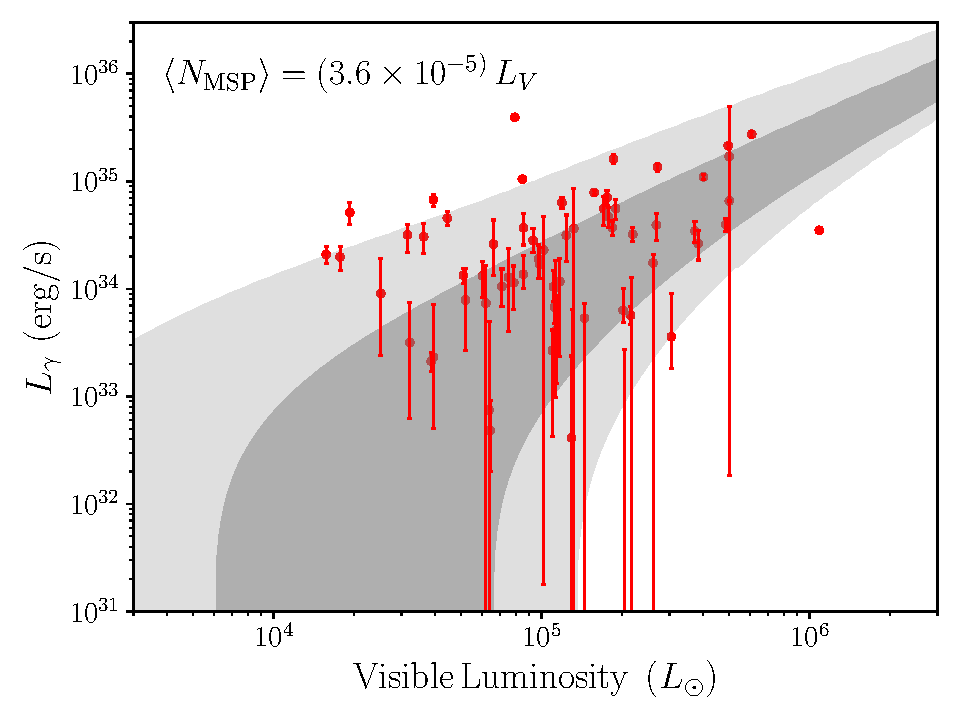
\includegraphics[width=0.49\textwidth]{sections/paper_msp/img/case3-dataplot.pdf}
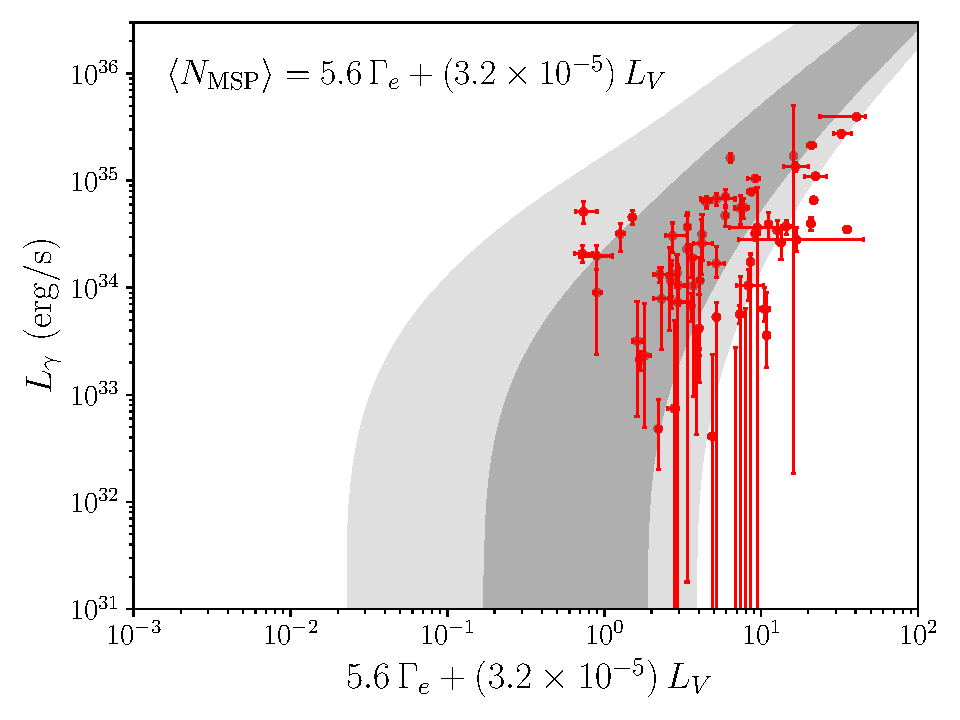
\includegraphics[width=0.49\textwidth]{sections/paper_msp/img/case4-dataplot.pdf}
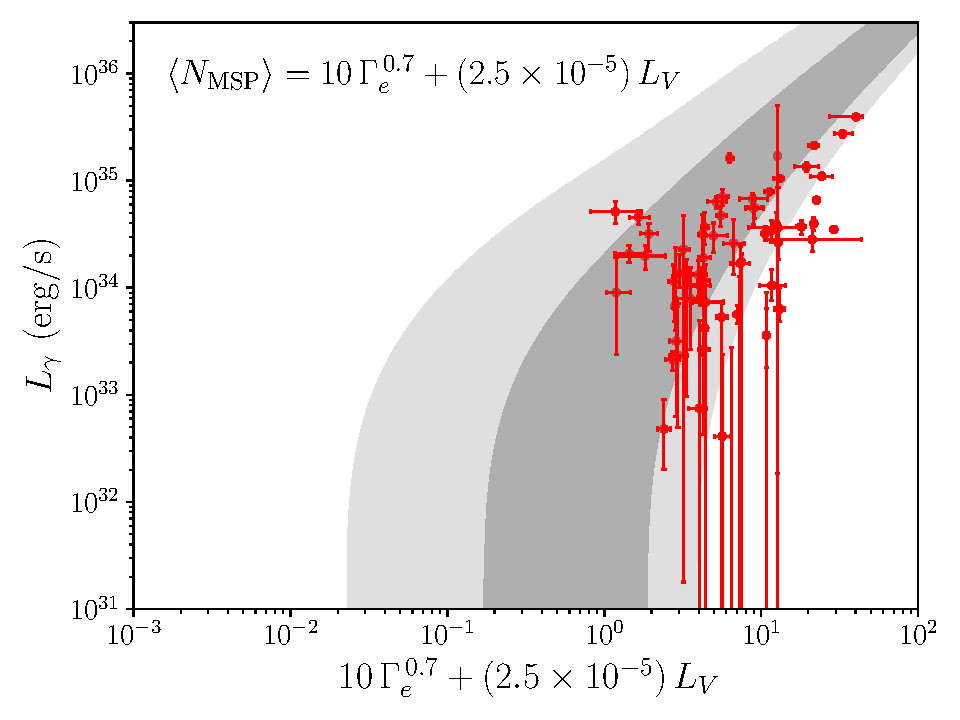
\includegraphics[width=0.49\textwidth]{sections/paper_msp/img/case5-dataplot.pdf}
\caption{The measured gamma-ray luminosities of the 87 globular clusters considered in this study (those with $L_V > 10^5 \, L_{\odot}$ or $\Gamma_e > 0.01$), compared to combinations of their stellar encounter rates and/or visible luminosities. As dark (light) grey bands, we show the 68.27\% (95.45\%) confidence interval predicted by the model for the the total gamma-ray luminosity. In each frame, we show the results that were obtained using the best-fit values for $\langle L_{\gamma} \rangle$, $\sigma_L$, $R_\textrm{MSP}$, and/or $R'_\textrm{MSP}$ (see Table~\ref{tab:param_constraints}).}
\label{fig:gamma1}
\end{figure}



In Figure~\ref{fig:gamma1}, we show several examples of the results we obtain following this procedure. In each frame, we plot the measured gamma-ray luminosities of the 87 globular clusters considered in this portion of our study (those with $L_V > 10^5 \, L_{\odot}$ or $\Gamma_e > 0.01$), compared to their stellar encounter rates, visible luminosities, or selected combinations thereof. Then, as dark (light) grey bands, we plot the 68.27\% (95.45\%) range of the total gamma-ray luminosity from a given cluster that is predicted by the model in question. In each frame, we show the results as found adopting the best-fit values for $\langle L_{\gamma} \rangle$, $\sigma_L$, $R_\textrm{MSP}$, and/or $R'_\textrm{MSP}$ (see Table~\ref{tab:param_constraints}).




\begin{figure}[t]
\centering
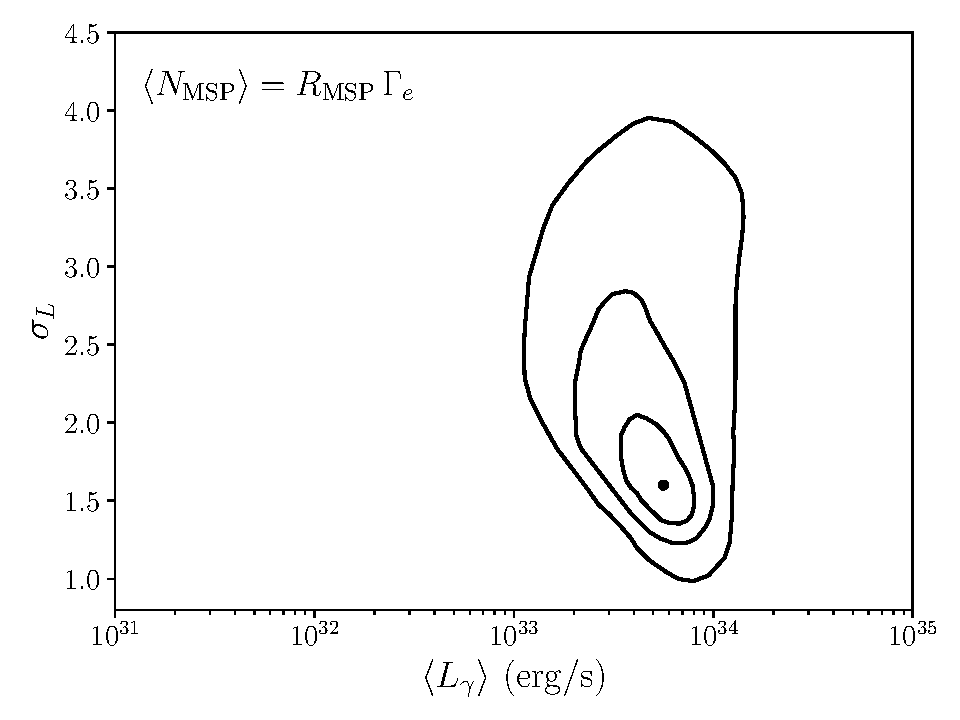
\includegraphics[width=0.49\textwidth]{sections/paper_msp/img/case1.pdf}
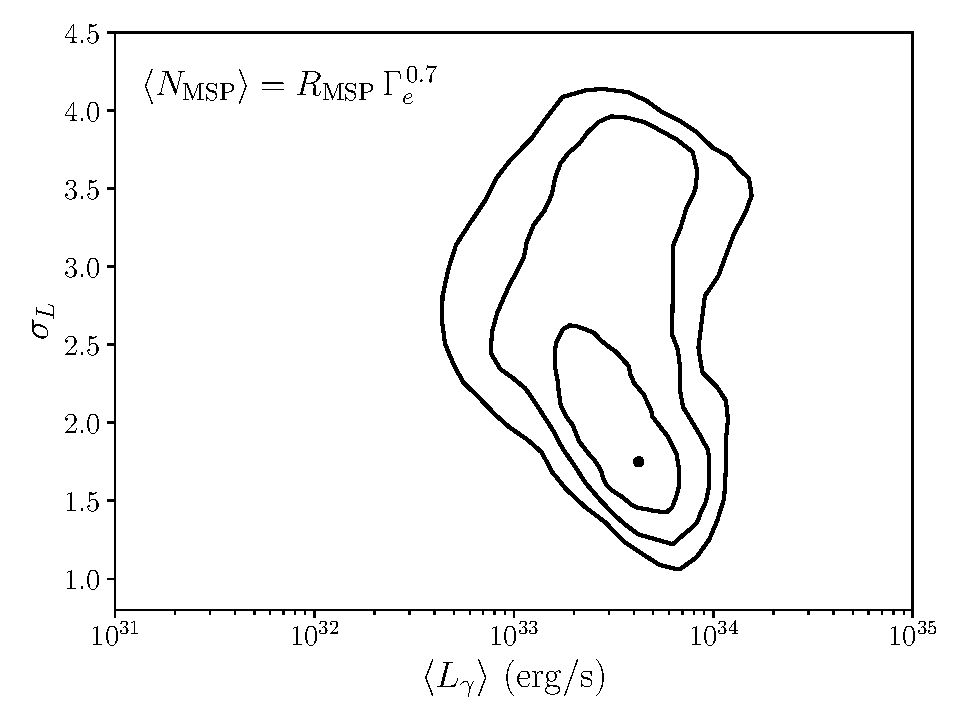
\includegraphics[width=0.49\textwidth]{sections/paper_msp/img/case2.pdf}
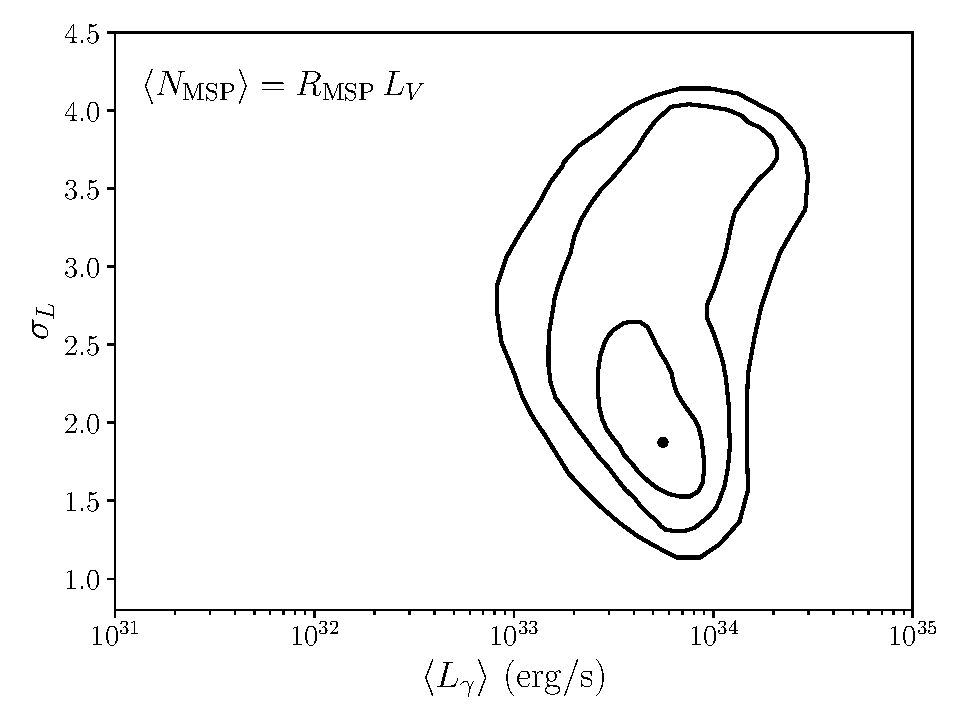
\includegraphics[width=0.49\textwidth]{sections/paper_msp/img/case3.pdf}
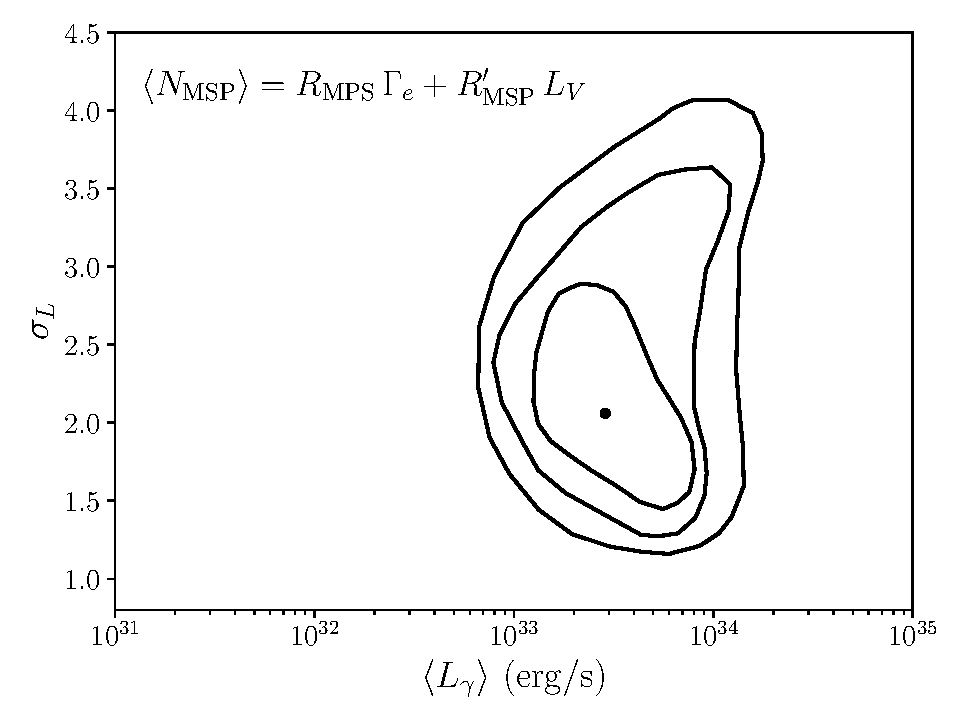
\includegraphics[width=0.49\textwidth]{sections/paper_msp/img/case4.pdf}
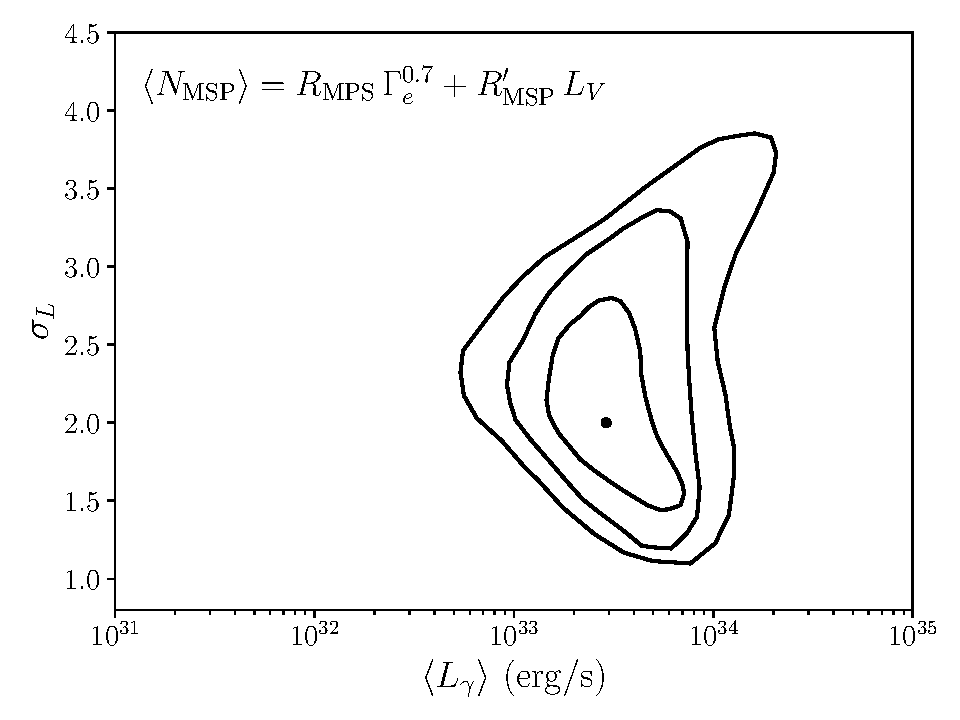
\includegraphics[width=0.49\textwidth]{sections/paper_msp/img/case5.pdf}
\caption{Constraints on the MSP gamma-ray luminosity function parameters, after marginalizing over $R_\textrm{MSP}$ and/or $R'_\textrm{MSP}$. The best-fit point in each frame is shown as a dot, while the contours reflect the regions that are preferred at the levels of 1, 2 and 3$\sigma$ confidence.}
\label{fig:constraints}
\end{figure}


In Figure~\ref{fig:constraints}, we plot the constraints on the luminosity function parameters, $\langle L_{\gamma} \rangle$ and $\sigma_L$, after marginalizing over the values of $R_\textrm{MSP}$ and/or $R'_\textrm{MSP}$. The best-fit point in each frame is shown by a dot, while the contours reflect the regions that are preferred at the levels of 1, 2 and 3$\sigma$ confidence. We show the results for each of the five hypotheses described in Section~\ref{sec:cases} for the relationship between the value of $\langle N_\textrm{MSP}\rangle$ and those of $L_V$ and/or $\Gamma_e$, finding each case to yield qualitatively similar results. Namely, this procedure consistently favors scenarios with $\langle L_{\gamma}\rangle \sim (1-8)\times 10^{33}\, \textrm{erg/s}$ and $\sigma_L \sim 1.4-2.7$. In Table~\ref{tab:param_constraints}, we show the values of the parameters favored by our analysis, including those for $R_\textrm{MSP}$ and $R'_\textrm{MSP}$. These parameters are directly related to the total number of gamma-ray MSPs contained within this sample of 87 globular clusters:  $N^\textrm{tot}_\textrm{MSP}=42.4 \, R_\textrm{MSP} + 1.55 \times 10^7 \, R'_\textrm{MSP}$ (for cases with $\langle N^\textrm{tot}_\textrm{MSP} \rangle \propto \Gamma_e$), or $N_\textrm{MSP}=41.7 \, R_\textrm{MSP}^{0.7} + 155 \times 10^7 \, R'_\textrm{MSP}$ (for cases with $\langle N_\textrm{MSP} \rangle \propto \Gamma_e^{0.7}$). For the parameters favored by our analysis, these 87 globular clusters contain a total of $\sim 400-1500$ gamma-ray emitting MSPs.

We note that the different hypotheses we have considered for the relationship between the value of $\langle N_\textrm{MSP}\rangle$ and those of $L_V$ and/or $\Gamma_e$ can yield significantly different values for the overall likelihood. In Table~\ref{tab:models_compare}, we show the difference between these resulting likelihoods (for the best-fit parameters in each case). Note that these hypotheses have different numbers of degrees-of-freedom, and this should be taken in to account when comparing their relative likelihoods.



\begin{table*}[t]
\centering
\normalsize
\vspace{12pt}
{\renewcommand{\arraystretch}{1.2}
\begin{tabular}{|c|c|cccc|}
    \hline $\langle N_\textrm{MSP}\rangle$ & Parameter & Best Fit & $\bm{1 \sigma}$ Range & $\bm{2 \sigma}$ Range & $\bm{3 \sigma}$ Range\\
    \hline\hline
      & $\langle L_{\gamma} \rangle$ & $5.6 \times 10^{33}$& $(3.4 - 8.1) \times 10^{33}$& $(2.0 - 10) \times 10^{33}$& $(1.1 - 13) \times 10^{33}$\\
      $R_\textrm{MSP} \, \Gamma_e$ & $\sigma_L$ & $1.6$& $1.4 - 2.0$& $1.2 - 2.8$& $1.0 - 3.9$ \\
    & $R_\textrm{MSP}$ & $11$& $9.5 - 15$& $7.6 - 32$& $6.4 - 110$ \\
    \hline
         & $\langle L_{\gamma} \rangle$ & $4.2 \times 10^{33}$& $(1.8 - 6.6) \times 10^{33}$& $(0.8 - 9.2) \times 10^{33}$& $(0.4 - 15) \times 10^{33}$\\
     $R_\textrm{MSP} \, \Gamma_e^{\,0.7}$ & $\sigma_L$ & $1.8$& $1.4 - 2.6$& $1.1 - 3.9$& $1.0 - 4.1$ \\
    & $R_\textrm{MSP}$ & $15$& $11 - 36$& $8.5 - 130$& $7.1 - 220$ \\
    \hline
         & $\langle L_{\gamma} \rangle$ & $5.6 \times 10^{33}$& $(2.7-8.7) \times 10^{33}$& $(1.4 - 21) \times 10^{33}$& $(0.8 - 29) \times 10^{33}$\\
     $R_\textrm{MSP} \, L_V$ & $\sigma_L$ & $1.9$& $1.5 - 2.7$& $1.3 - 4.0$& $1.1 - 4.1$ \\
    & $R_\textrm{MSP}$ & $3.6\times 10^{-5}$& $(2.7-6.5)\times 10^{-5}$& $(1.8-22)\times 10^{-5}$& $(1.4-35)\times 10^{-5}$ \\
    \hline    
%%%    
         & $\langle L_{\gamma} \rangle$ & $2.9 \times 10^{33}$& $(1.3 - 5.5) \times 10^{33}$& $(0.9 - 8.4) \times 10^{33}$& $(0.7 - 14) \times 10^{33}$\\
     $R_\textrm{MSP} \, \Gamma_e$ & $\sigma_L$ & $2.1$& $1.7 - 2.6$& $1.3 - 3.5$& $1.2 - 4.0$ \\
    $+R'_\textrm{MSP}\,L_V$& $R_\textrm{MSP}$ & $5.6$& $3.2 - 14$& $1.8 - 21$& $1.2 - 39$ \\
    & $R'_\textrm{MSP}$ & $3.2\times 10^{-5}$& $(1.8-8.0)\times 10^{-5}$& $(1.4-11)\times 10^{-5}$& $(1.1-18)\times 10^{-5}$ \\
    \hline   
%%%
         & $\langle L_{\gamma} \rangle$ & $2.9 \times 10^{33}$& $(1.4 - 7.2) \times 10^{33}$& $(0.9 - 8.7) \times 10^{33}$& $(0.5 - 21) \times 10^{33}$\\
     $R_\textrm{MSP} \, \Gamma_e^{0.7}$ & $\sigma_L$ & $2.0$& $1.4 - 2.8$& $1.2 - 3.4$& $1.1 - 3.9$ \\
    $+R'_\textrm{MSP}\,L_V$& $R_\textrm{MSP}$ & $10$& $6.4-23$& $3.9 - 66$& $2.9 - 110$ \\
    & $R'_\textrm{MSP}$ & $2.5\times 10^{-5}$& $(1.6-5.7)\times 10^{-5}$& $(1.1-8.0)\times 10^{-5}$& $(0.8-11)\times 10^{-5}$ \\
    \hline   
\end{tabular}
}
\caption{The parameter values favored by our analysis. Values for the average MSP gamma-ray luminosity, $\langle L_{\gamma} \rangle$, are given in erg/s.}
\label{tab:param_constraints}
\end{table*}

\begin{table*}[t]
\centering
\normalsize
\vspace{12pt}
{\renewcommand{\arraystretch}{1.2}
\begin{tabular}{|c|c|}
    \hline $\langle N_\textrm{MSP}\rangle$ & $-2\Delta \ln \mathcal{L}$\\
    \hline\hline
       $R_\textrm{MSP} \, \Gamma_e$ & 146.0 \\
    \hline
       $R_\textrm{MSP} \, \Gamma_e^{\,0.7}$ & 45.4 \\
    \hline
       $R_\textrm{MSP} \, L_V$ & 37.7 \\
    \hline    
       $R_\textrm{MSP} \, \Gamma_e +R'_\textrm{MSP}\,L_V$ & 13.5 \\
    \hline  
       $R_\textrm{MSP} \, \Gamma_e^{\,0.7} +R'_\textrm{MSP}\,L_V$ & 0.0 \\
    \hline      
\end{tabular}
}
\caption{The change in twice the log-likelihood of our analysis, relative to the best-fit case shown in the bottom row of this table.}
\label{tab:models_compare}
\end{table*}

So far, we have assumed that the mean number of MSPs in a given globular cluster is determined entirely by its luminosity and/or stellar encounter rate, without any departures from this prediction (other than the scatter inherent in each cluster's draw from the Poisson distribution for $N_\textrm{MSP}$). In reality, our models for determining $\langle N_\textrm{MSP} \rangle$ cannot possibly contain all of the relevant information and, therefore, should not be perfectly predictive. This leads us to expect that there should some degree of variation in the mean number of MSPs in given cluster, beyond that which can be predicted by the values of $L_V$ and $\Gamma_e$ alone. 

To assess the impact of such cluster-to-cluster variation, we take the mean number of expected MSPs to have an intrinsic degree of scatter, which we model according to a log-normal distribution with a width, $\sigma_N$. This more complex model represents a potentially more conservative approach, and allows us to accounting for potential unmodeled systematic uncertainties. By rerunning our analysis, we find that in the case of our best fit model, $\langle N_\textrm{MSP}\rangle = R_\textrm{MSP} \, \Gamma_e^{0.7} +R'_\textrm{MSP} \, L_V$, the overall fit is improved by a maximum of $-2\Delta \ln \mathcal{L} \approx 8$ for $\sigma_N \approx 0.5$. In this new best fit, the values of $\langle L_{\gamma} \rangle$ and $\sigma_L$ are shifted modestly from the case without this intrinsic scatter, from $\langle L_{\gamma} \rangle \approx 2.9 \times 10^{33} \, \textrm{erg/s}$ and $\sigma_L \approx 2.0$ to $\langle L_{\gamma} \rangle \approx 1.8\times 10^{33} \, \textrm{erg/s}$ and $\sigma_L \approx 1.4$.

While an improvement of $-2\Delta \ln \mathcal{L} \approx 8$ corresponds to a statistical preference between 2$\sigma$ and 3$\sigma$, this more complex model also introduces new modeling uncertainties. Given this, we cannot exclude that this improvement is due to statistical fluctuations or unknown systematic uncertainties. We therefore refrain from adopting the model with cluster-to-cluster variations as our fiducial baseline, and instead opt for the simpler fitting formula without variations, which has a stronger basis in the literature.



Before moving on, we will use these results to comment on the previous studies that have interpreted the gamma-ray emission observed from NGC 5139~\cite{Reynoso-Cordova:2019biv} and NGC 104~\cite{Brown:2018pwq} to be possible signals of annihilating dark matter. Although this interpretation cannot be easily ruled out, our results in Figure~\ref{fig:gamma1} demonstrate why no such exotic emission is required. In fact, these clusters have values of $\Gamma_e$ and $L_V$ that are entirely compatible with their observed gamma-ray luminosities. No dark matter annihilation or other exotic contributions are required.  

